\chapter{Implementation Part II: Enhancing Storage Format}
\label{chap:storage-format}
We continue our research by exploring how more memory can be saved by enhancing the storage format. First, we replace the \cn{GValue} as the main storage format and replace it with primitive data types. Then, we investigate whether these values can be passed directly and stored in the columns.

\section{Primitive Data Types}
\label{sec:Simple Data Types}
As we saw in the background section, delphi has several primitive data types. These include integer, boolean, character, and real value types. In this chapter, we also discuss record types and string types. The main benefit of these types is that they are not pointer types, and when you allocate memory for such value, the data itself is stored there, and not a pointer to the value. This does not apply to strings. Classes are allocated by the memory manager by calling \fn{Create}, but using simple data types, we explicitly allocate memory for the data. Hence, a transition from \cn{GValue} to simple data types should give us more control over memory.

We also saw that there was a significant overhead in a class type in \delphi. For each \cn{GValue}, there was a 20 byte overhead in pointers and reference counting. In comparison, the \cn{boolean} data type in \delphi~only uses 1 byte.

Motivated by the memory reduction and potential to regain control over memory, we create a new structure using the same interface as \cn{FieldValueCollection}, which we denote as \cn{PrimitiveFieldValueCollection}, that stores data as primitive data values, and not as \cn{GValue}s.

\section{PrimitiveFieldValueCollection}
\label{sec:PrimitiveFieldValueCollection}
We propose to not store \cn{GValue} instances within the columns, but rather as primitive data types. However, since the column operations still uses \cn{GValue} in its access methods, the data has to be extracted from these instances on its way in, and new \cn{GValues} must be created on the way out. In this research, we refer to these simple data types an \textit{Primitive Data Types}.

\afigure{img/primitive-hierarchy.png}{Primitive hierarchy}{fig:primitive-hierarchy}{1.0}
The new column structure is implemented with a generic base class, and a subclass for every supported date type. The base class inherits from \cn{FieldValueCollectionBase}, which is the base class and interface for all field value collection columns. The hierarchy is shown in Figure \ref{fig:primitive-hierarchy}.

\begin{delphicode}{\fn{GetValue} function in \cn{PrimitiveFieldValueCollectionBase}.}{lst:primitive-get-value}
function PrimitiveFieldValueCollectionBase<TType>.GetValue
( index : integer )
: CGValue;
begin
  EnsureCapacity(index);
  if not nilFlags[index] then
    Result := valueHelper.CreateCGValue(values[index])
  else
    Result := nil;
end;
\end{delphicode}

To help isolate all code related to value conversion, we create a value helper class that is instantiated for the various data types. This class contains methods for extracting a primitive data value from a \cn{GValue}, creating a \cn{GValue} based on a primitive data type. Its usage is seen in Listing \ref{lst:primitive-get-value}. The class is generic, with subclasses for every supported data type, and is owned by the \cn{PrimitiveFieldValueCollectionBase} class.

The \vn{nilFlags} bitmap is important in this class. Whereas \texttt{null} could have been indicated by null pointers in the original column implementations, primitive data types has no such value. Although variants in \delphi~could have been used to solve the issue, such that primitive data values could be assigned \texttt{null}, this generates an extra overhead. Hence, the bitmap is used to indicate which values are null. As seen in Listing \ref{lst:primitive-get-value}, the flags are checked prior to creating a value.

Even though they are not considered primitive data types, we apply the same techniques for strings and records. Record types, like \vn{TGuid} and \vn{SCalendarTime}, works similarly as primitive data types, which means they will be allocated consecutive in memory in the \cn{TArray} structure. Strings, however, are pointer types, which means that only pointers will be stored in the columns. Hence, we dont get the benefit from explicit memory control, but we do remove an extra layer of indirection to access a value, and we avoid the overhead related to \cn{GValue}.

\subsection{Column Selector}
\label{sub:Column Selector}
To make the new \cn{PrimitiveFieldValueCollection} class work, correct columns must be chosen for different data descriptors. Hence, \cn{CompositionValueCollection}, or the column store, was expanded with a \fn{GetFieldValueCollection}. This method inputs a data descriptor and returns a pointer to a new column structure. In this method, the data descriptor is queried for its type, and the correct \cn{PrimitiveFieldValueCollectionBase} subclass is returned. If no matching primitive data type column is found, the column selector falls back on the original \cn{FieldValueCollection} from Chapter \ref{chap:column-store}.

\section{Avoiding GValues at Load Time}
\label{sec:Avoiding GValues at Load Time}
\begin{figure}
    \centering
    \begin{subfigure}{\textwidth}
        \centering
        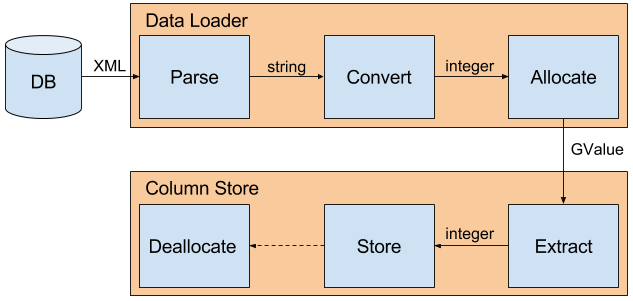
\includegraphics[width=\textwidth]{img/gap-load-original.png}
        \caption{Original implementation where all data is transferred as \cn{GValue}s.}
    \end{subfigure}
    \begin{subfigure}{\textwidth}
        \centering
        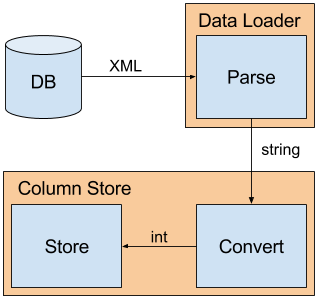
\includegraphics[width=0.5\textwidth]{img/gap-load-raw.png}
        \caption{Enhanced implementation where data is passed to the column store as strings.}
    \end{subfigure}
\caption{By letting the column store accept raw string values from XML, the load process is simplified, and uneccessary memory allocations for \cn{GValues} are removed.}
\label{fig:gap-load-raw}
\end{figure}

In \gap, composition objects in a data source are filled with data using a loading mechanism found in the core event handler. This loader queries the database server and accepts XML values. The loader parses the XML and creates \cn{GValue}s which in turn is sent to the composition objects. Our observation is, with the primitive data type column implementation, that creating \cn{GValue}s when loading a data mart is no longer needed, and that simple type conversions from string would suffice. This is illustrated in Figure \ref{fig:gap-load-raw}.

\begin{delphicode}{\fn{SetXMLValue} in \cn{PrimitiveFieldValueCollectionBase}.}{lst:primitive-set-xml-value}
procedure PrimitiveFieldValueCollectionBase<TType>.SetXMLValue
( index : integer; xmlValue : string);
begin
  EnsureCapacity(index);
  values[index] := valueHelper.GetFromXMLValue(xmlValue);
  nilFlags[index] := FALSE;
  assignedFlags[index] := TRUE;
end;
\end{delphicode}

To do this, \cn{FieldValueCollectionBase} is extended with a method \cn{LoadXMLValue} that accepts an index and a string xml value. The value helper class is also extended correspondingly, with high performance value conversion functions from the standard library, like \fn{StrToInt} and \fn{StrToFloat}. For more advanced data types, like date, the correct parser functions are called. The implementation is seen in Listing \ref{lst:primitive-set-xml-value}.

We hypothesize that loading xml values directly into a column will speed up load time. We believe this is the case because there will be no allocation and deallocation of \cn{GValues}. Also, as seen in Figure \ref{fig:gap-load-raw}, the new implementation has less steps than the original.

\section{Test Results}
\label{sec:Test Results}
Like last chapter, we test our implementation with Benchmark \ref{bm:q1} and Benchmark \ref{bm:write}. We are curious to see whether memory has been reduced by avoiding the overhead corresponding with \cn{GValue}s and whether load time has been affected. Write performance is also important to test, since \cn{GValue}s are allocated and deallocated as they are read and written to the columns. Full descriptions of the benchmarks are found in Appendix \ref{app:bm}.

\subsection{TPC-H Result}
\label{sub:TPC-H Result}
Benchmark \ref{bm:q1}, the \textit{TPC-h Q1 Data Load Benchmark}, was run with our new primitive value column implementation with and without the new loading scheme. Both scaling factor 0.1 and 0.01 were run. Like in Chapter \ref{chap:column-store}, only three tests were run per configuration. However, all results yielded low variance, and no single measurement was more than 15 \% different than the average value.

\begin{table}
    \centering
    \begin{tabularx}{\textwidth}{X | X X}
        & SF0.01 & SF0.1 \\ 
        \hline
        \hline
        Column Store & 419 bytes & 501 bytes \\
        Primitive Column Store & 333 bytes & 374 bytes \\
        Primitive Column Store /w raw load & 381 bytes & 422 bytes \\
    \end{tabularx}
    \caption{Bytes per \texttt{LINEITEM} used by the new primitive value implementation.} 
    \label{tab:primitive-bpl}
\end{table}
As seen in Table \ref{tab:primitive-bpl}, memory is reduced from 419 to 333 bytes and from 501 to 374 bytes for scaling factors 0.01 and 0.1 respectively. This corresponds to 21 \% and 25 \% reduced memory footprint. However, our new loading mechanism increases memory consumption.

\begin{table}
    \centering
    \begin{tabularx}{0.75\textwidth}{X | X X}
        & SF0.01 & SF0.1 \\ 
        \hline
        \hline
        Column Store & 842 ms & 8539 ms \\
        Primitive Column Store & 1210 ms & 13585 ms \\
        Primitive Column Store w/ raw load &  20966 ms & 2306 ms \\
    \end{tabularx}
    \caption{Load times for Benchmark \ref{bm:q1} for the primitive column store for scaling factors 0.01 and 0.1.} 
    \label{tab:primitive-load}
\end{table}
Load times were increased by the primitive column store, but it is still lower than the original implementation. However, with our new loading mechanisms, the load time has increased even more, and is very close to the original implementation. The results are shown in table \ref{tab:non-blackbox-load}. We are surprised to see that our new loading mechanism has degraded load performance. We discuss this in greater detail in Section \ref{sec:part2-discussion}. 

\begin{table}
    \centering
    \begin{tabularx}{\textwidth}{X | X X X | X X X X}
        & \multicolumn{3}{c}{Lookup Index} & \multicolumn{4}{c}{Source Measure Lookup} \\
        \hline
        \hline
        Column Store & 3123 ms & 3301 ms & 13004 ms & 532 ms & 625 ms & 646 ms & 752 ms \\
        Primitive Column Store & 11393 ms & 11960 ms & 19365 ms & 6556 ms & 6856 ms & 6840 ms & 6826 ms \\
    \end{tabularx}
    \caption{Data mart load operation times for \ref{bm:q1} with the primitive columns.} 
    \label{tab:primitive-q1}
\end{table}
Most operations are drastically slowed down by the new primitive storage format, as seen in Table \ref{tab:primitive-q1}. Source measure lookup is ten times slower than the previous column store implementation, and almost 20 times slower as the original implementation.

\subsection{Write Benchmark}
\label{sub:Write Benchmark}
\begin{table}
    \begin{tabularx}{\textwidth}{X | X X X X}
         & \texttt{QUANTITY} & \texttt{EXTENDEDPRICE} & \texttt{COMMENT} & \texttt{SHIPDATE}\\ 
        \hline
        \hline
        Column Store & 1642 ms & 1610 ms & 1770 ms & 2046 ms \\
        Primitive Column Store & 1807 ms & 1779 ms & 1820 ms & 2352 ms \\
    \end{tabularx}
    \caption{Test results for Benchmark \ref{bm:write}.}
    \label{tab:primitive-write}
\end{table}
Write performance has, as Table \ref{tab:primitive-write} shows, degraded slightly with the new primitive data type column store. No operations are more than 15 \% slower than the original.

\section{Discussion}
\label{sec:part2-discussion}
We are happy to see that memory have been reduced by up to 25 \% for SF0.1. This means the overhead associated with \cn{GValues} is significant, and by storing data as primitive data types, this is removed. Load time has been increased from the original column store implementation, and we believe this is caused by the extra steps needed to extract the primitive data type from \cn{GValue}s. Keep in mind that load time still is lower than the original row-store implementation in \gap.

Both lookup index generation and loading of source measure lookup performance has been reduced. For the latter, the operation takes 10 times longer, or 20 times longer as the original. We believe these operations are affected because they work on data in tight loops, that is, little more than accessing values is done. For each iteration, a \cn{GValue} is created, value is extracted, and the instance is deallocated again. In the original implementation, the \cn{GValues} were already present, and only the pointers had to be passed out.

The extra steps of \cn{GValue} allocation and deallocation also affects write performance in Benchmark \ref{bm:write}, although not by more than 15 \%. This indicates that there are much more overhead associated with data write than just allocating \cn{GValue}s.

\section{Chapter Conclusion}
\label{sec:Chapter Conclusion}
Write performance have only suffered slightly by storing data as primitive data types. We are, therefore, confident that even more compression can happend behind the scenes in the columns, and that using an interface with \cn{GValue}s is feasible. 

Yet to be explored is that we have regained control over alignment in memory. Now, that all types are stored in an array structure with primitive data types, we may increase processor throughput. For instance, both lookup index and source measure lookup creation has become much slower. We claim that these operations can be speeded up by working on the arrays directly. We investigate these operations in Chapter X.

\subsection{Future Work}
\label{sub:Future Work}
We see a potential in loading XML values directly, however our implementation did nothing but decrease performance since the caching mechanisms was disabled. A more thorough implementation is outside of the scope of this research. Future work should investigate the effects of loading XML data directly into the columns and have the column store handle all caching using dictionary encoding. In theory, all caching should be handled by the column store using a loading state.
